\beginsong{Möge die Straße}[
    wuw={nach einem irischen Volkslied},
    % kssiv={326},
    % siru={164},
    % biest={611},
    % egplus={37},
]

\beginverse
\[F]Möge die \[C]Straße \[Dm]uns zusammen \[Am]führen
\[H&]und der Wind in \[F]deinem Rücken \[C]sein.
\[F]Sanft falle \[C]Regen \[Dm]auf deine \[Am]Felder
und \[H&]warm auf dein Ge\[C]sicht der Sonnen\[F]schein. \[F7]
\endverse

%\centering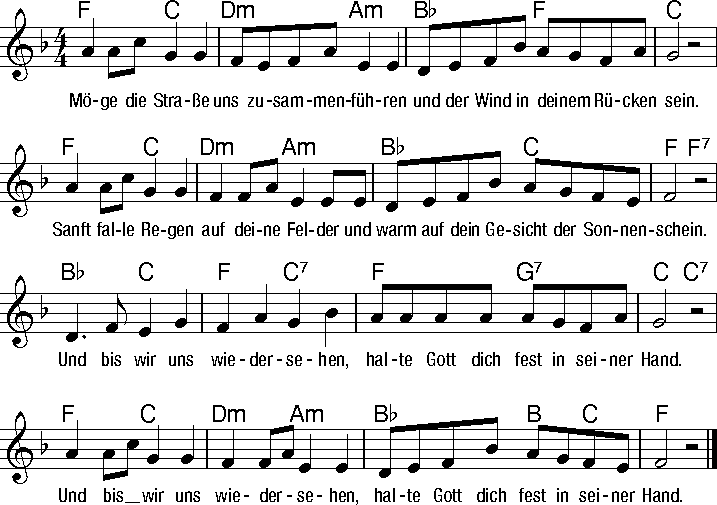
\includegraphics[width=1\textwidth]{Noten/Lied115.pdf}

\beginchorus
\[H&]Und bis \[C]wir uns \[F]wieder\[C7]sehen
\[F]halte Gott dich \[G7]fest in seiner \[C]Hand. \[C7]
\endchorus

\beginverse
^Führe die ^Straße, ^die du ^gehest,
^immer nur zu ^deinem Ziel bergab;
^Hab, wenn es ^kühl wird ^warme Ge^danken 
^und den vollen ^Mond in dunkler ^Nacht. ^
\endverse

\beginverse
^Hab' unterm ^Kopf ein ^weiches ^Kissen,
^habe Kleidung ^und das täglich ^Brot;
^Sei über ^40 ^Jahre im ^Himmel,
be^vor der Teufel ^merkt: Du bist schon ^tot. ^
\endverse

\beginverse
^Bis wir ^uns mal ^wieder^sehen,
^hoffe ich, dass ^Gott dich nicht ver^lässt;
^Er halte ^dich in ^seinen ^Händen,
^drücke seine ^Faust dich nicht zu ^fest.
\endverse

\endsong
